%% ============================================================
%%  Chapter 1 — Project Framework
%% ============================================================
\begingroup
\renewcommand{\baselinestretch}{0.85}
\chapter{Project Framework}
\minitoc
\endgroup
\newpage

%% ------------------------------------------------------------
\section*{Introduction}
\addcontentsline{toc}{section}{Introduction}
%% ------------------------------------------------------------

This chapter presents the general framework of the \textbf{Tesla Academy} project.
It first introduces the context and motivation behind the project, then presents the host
organization and its main activities. It also provides an analysis of the existing situation
in the online learning market, followed by a comparative study of relevant learning
platforms. Finally, the proposed solution is described, along with the project management
methodology adopted during the development process.

%% ------------------------------------------------------------
\section{Context and Motivation}
%% ------------------------------------------------------------

The rapid growth of the Internet and the widespread use of connected devices have deeply
transformed educational practices worldwide. Online learning, commonly known as
\textit{e-learning}, has become an important approach for delivering accessible, flexible,
and personalized learning experiences.

In Tunisia and across the MENA region, educational and training institutions, including
public universities, private schools, professional training centers, and independent
instructors, are increasingly seeking digital solutions to modernize their educational
processes. These solutions are needed in order to:

\begin{itemize}
  \item Extend educational offers beyond geographical and time constraints, reaching a
        wider audience;
  \item Improve learner monitoring through dashboards, progress tracking, and reporting
        tools;
  \item Reduce the operational costs related to the administrative management of training
        activities;
  \item Provide online assessments and certifications in a structured and reliable way.
\end{itemize}
However, many existing Learning Management System (LMS) solutions available on the market,
such as Moodle, TalentLMS, and Udemy Business, may present limitations in the Tunisian and
regional context. These limitations include high customization or deployment complexity,
limited support for local payment gateways, insufficient flexibility for managing multiple
organizations within the same system, and interfaces that are not always fully adapted to
the linguistic and organizational needs of local users.

Recognizing these challenges, YohaTech identified an opportunity to develop a digital
learning platform dedicated to educational institutions, training centers, independent
instructors, and learners. The objective was to create a solution capable of addressing
the limitations of existing platforms while providing a modern, scalable, and intelligent
learning environment adapted to the needs of the Tunisian and regional market.

In this context, the \textbf{Tesla Academy} project was initiated as part of a final-year
internship at \textbf{YohaTech Monastir}, in partial fulfillment of the requirements for the
National Engineering Degree in Computer Science, specializing in Software Engineering, at
ISIMM. The objective of this project is to design and develop a \textit{Made in Tunisia}
AI-powered multi-organization LMS platform that allows several organizations to coexist
within a shared technological infrastructure while maintaining isolated, secure, and
customizable workspaces.

%% ------------------------------------------------------------
\section{Presentation of the Host Organization}
%% ------------------------------------------------------------

\subsection{YohaTech Monastir}

\begin{figure}[htbp]
  \centerline{
\includegraphics[scale=0.40]{logoyohatech.png}}
  \caption{YohaTech Monastir Logo}
  \label{fig:yohatech_logo}
\end{figure}

YohaTech is a Tunisian technology start-up based in Monastir. The company operates in
several technological fields, including intelligent systems, robotics, embedded electronics,
and software development. It combines mechanical engineering, electronics, and computer
science to design innovative solutions adapted to modern industrial, residential, and
educational needs.

The company develops solutions involving embedded systems, customized electronic boards,
software applications, and Internet of Things (IoT) technologies. YohaTech is also active in
industrial robotics, automation, and smart home solutions.

Through a multidisciplinary and innovation-oriented approach, YohaTech supports its clients
in the design and development of high-value technological solutions across different sectors.

\subsection{Services}

The main services provided by YohaTech include:

\begin{itemize}
  \item \textbf{Software development}: design and development of web applications,
        mobile applications, and custom software solutions;

  \item \textbf{Embedded electronics}: development of electronic boards, embedded
        systems, and microcontroller-based solutions;

  \item \textbf{Robotics and automation}: design of robotic systems and industrial
        automation solutions;

  \item \textbf{Internet of Things (IoT)}: integration of connected objects and
        intelligent solutions for smart homes and industrial environments;

  \item \textbf{Mechatronic solutions}: combination of mechanics, electronics, and
        software to develop intelligent systems;

  \item \textbf{Technology consulting}: technical guidance in choosing suitable hardware
        and software architectures for innovative projects.
\end{itemize}

%% ------------------------------------------------------------
\section{Study of the Existing Situation}
%% ------------------------------------------------------------

This section analyzes the current state of online learning and training management
platforms in order to identify the challenges faced by educational institutions, training
centers, and independent instructors. The objective is to highlight the limitations of
existing solutions and justify the development of Tesla Academy.

\subsection{Current Situation}

The rapid digitalization of education has led to the widespread adoption of Learning
Management Systems (LMS) and online learning platforms. Educational institutions, training
centers, and independent instructors increasingly rely on digital solutions to deliver
educational content, manage learners, conduct assessments, and monitor learning progress.

Several LMS platforms currently exist on the market, ranging from open-source solutions
such as Moodle to commercial platforms such as TalentLMS, Blackboard, Canvas, and Udemy
Business. These solutions provide a variety of functionalities, including course management,
assessments, learner tracking, communication tools, and certification management.

Despite their popularity, many existing platforms are designed primarily for a single
organization or a specific educational context. Consequently, organizations often encounter
difficulties when attempting to manage multiple entities, customize their learning
environments, integrate local services, or provide intelligent learning assistance to users.

\subsection{Existing Functionalities}

Most modern LMS platforms provide a common set of educational functionalities, including:

\begin{itemize}
  \item Course and learning content management;
  \item Learner enrollment and user management;
  \item Online quizzes, assignments, and assessments;
  \item Progress monitoring and reporting;
  \item Certification and completion tracking;
  \item Communication and collaboration tools;
  \item Integration with video conferencing platforms.
\end{itemize}

These functionalities provide a solid foundation for digital learning and have contributed
significantly to the growth of online education worldwide.

\subsection{Strengths of Existing Solutions}

The analysis of current LMS platforms reveals several strengths:

\begin{itemize}
  \item Widespread adoption and proven effectiveness in educational environments;
  \item Availability of rich course management and assessment features;
  \item Support for remote and hybrid learning models;
  \item Availability of reporting and learner tracking mechanisms;
  \item Integration with various third-party services and educational tools.
\end{itemize}

\subsection{Weaknesses and Limitations}

Despite their advantages, existing solutions still present several limitations, particularly
in the context of the Tunisian and regional educational market:

\begin{itemize}
  \item \textbf{Limited multi-organization support}: many platforms are not designed to
        efficiently manage multiple organizations through isolated and customizable
        workspaces within a single platform;

  \item \textbf{High deployment and customization costs}: advanced LMS solutions often
        require significant financial investment and technical expertise;

  \item \textbf{Limited integration with local payment systems}: support for Tunisian
        payment gateways such as Konnect and Paymee is generally unavailable;

  \item \textbf{Insufficient localization}: some platforms offer limited support for
        regional languages and local educational requirements;

  \item \textbf{Fragmented learning experience}: learners and instructors frequently depend
        on multiple external tools to complete their activities;

  \item \textbf{Limited Artificial Intelligence integration}: many traditional LMS
        platforms provide little or no support for intelligent tutoring, automated question
        generation, assignment feedback, content retrieval, and personalized learning
        assistance;

  \item \textbf{Scalability and flexibility challenges}: adapting existing solutions to
        different organizational structures and educational business models may be complex
        and costly.
\end{itemize}

%% ------------------------------------------------------------
\section{Benchmark of Existing Solutions}
%% ------------------------------------------------------------

This section presents a comparative study of existing LMS and e-learning solutions. The
objective is to identify their strengths and limitations in order to guide the design
choices of Tesla Academy.

\subsection{Selected Solutions}

Three representative platforms were selected based on their relevance to the target market
and their positioning in the field of online learning.

\subsubsection{Solution 1: TalentLMS}

\begin{figure}[htbp]
  \centerline{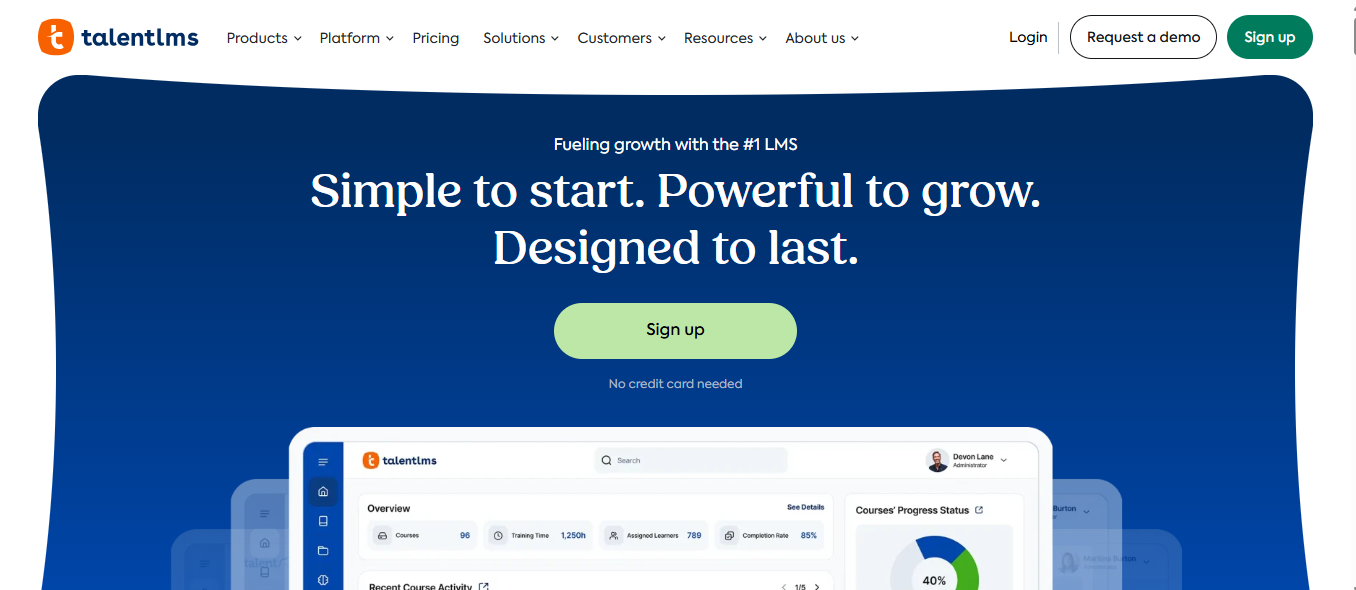
\includegraphics[scale=0.35]{talentlms_screenshot.png}}
  \caption{TalentLMS Interface}
  \label{fig:talentlms}
\end{figure}

TalentLMS is a cloud-based LMS widely used in the professional training sector. One of its
main strengths is the concept of branches, which allows organizations to create separated
training environments with specific users, courses, and branding. TalentLMS also provides
an intuitive interface and integration capabilities. However, in the Tunisian context, its
adoption may be limited by pricing constraints, dependence on external services, and the
lack of native support for local payment gateways.

\subsubsection{Solution 2: Udemy Business}

\begin{figure}[htbp]
  \centerline{
\includegraphics[scale=0.35]{udemy_screenshot.png}}
  \caption{Udemy Business Homepage}
  \label{fig:udemy}
\end{figure}

Udemy Business is the professional version of the Udemy platform. It gives organizations
access to a large catalog of online courses covering many fields. Its main strength lies in
the richness of its content library and the quality of its marketplace model. However, it
offers limited control over course creation, platform customization, and
organization-specific workflows. It is also less suitable for institutions that need to
manage their own trainers, learners, assessments, payments, and internal educational
processes.

\subsubsection{Solution 3: TakiAcademy}

\begin{figure}[htbp]
  \centerline{
\includegraphics[scale=0.35]{takiacademy_screenshot.png}}
  \caption{TakiAcademy Homepage}
  \label{fig:takiacademy}
\end{figure}

TakiAcademy is a Tunisian e-learning platform mainly oriented toward primary and secondary
education. It provides educational content aligned with the Tunisian national curriculum and
offers an interface adapted to young learners. However, it is not primarily designed for
multi-organization management, higher education, professional training centers, or
independent instructors who need advanced administrative and pedagogical control.

\subsection{Comparative Table}

\begin{table}[htbp]
\centering
\caption{Comparison of Existing Solutions}
\label{tab:benchmark}

\renewcommand{\arraystretch}{1.3}

\begin{tabularx}{\textwidth}{
|>{\raggedright\arraybackslash}X
|>{\centering\arraybackslash}m{2.5cm}
|>{\centering\arraybackslash}m{3cm}
|>{\centering\arraybackslash}m{2.5cm}|}
\hline

\textbf{Criterion}
& \textbf{TalentLMS}
& \textbf{Udemy Business}
& \textbf{TakiAcademy} \\
\hline

Multi-organization management
& \checkmark
& \texttimes
& \texttimes \\
\hline

Support for Tunisian local payment gateways
& \texttimes
& \texttimes
& \checkmark \\
\hline

French / Arabic language support
& Partial
& Partial
& \checkmark \\
\hline

Public course catalog
& \texttimes
& \checkmark
& \checkmark \\
\hline

Advanced quiz and assessment management
& \checkmark
& Partial
& Partial \\
\hline

Integrated live sessions
& Partial
& \texttimes
& Partial \\
\hline

AI-powered learning features
& Partial
& Partial
& \texttimes \\
\hline

Platform customization
& \checkmark
& \texttimes
& Partial \\
\hline

Adaptation to the Tunisian market
& Partial
& Partial
& \checkmark \\
\hline

\end{tabularx}
\end{table}

Table~\ref{tab:benchmark} highlights the main limitations of existing solutions in relation
to the needs of the Tunisian and regional educational market. While some platforms provide
advanced learning features, they may lack local payment support, advanced customization,
multi-organization flexibility, or AI-powered tools adapted to the target users.

%% ------------------------------------------------------------
\section{Proposed Solution}
%% ------------------------------------------------------------

\textbf{Tesla Academy} is an AI-powered multi-organization Learning Management System
designed to meet the needs of educational institutions, training centers, independent
instructors, and learners. The platform aims to provide a unified environment for managing
online learning activities while ensuring flexibility, scalability, and secure separation
between organizations.

The proposed solution is based on the following main principles:

\begin{itemize}
  \item \textbf{Multi-organization architecture}: each organization, such as a university,
        training center, or private school, has its own isolated workspace, identity,
        users, courses, and administrative environment;

  \item \textbf{Multiple user profiles}: the platform supports several roles, including
        Super Administrator, Organization Administrator, Instructor, and Student, each
        with a dedicated dashboard and specific permissions;

  \item \textbf{Public course catalog}: in addition to private organizational spaces, a
        public catalog allows independent learners to access selected courses offered
        through the platform;

  \item \textbf{Local payment integration}: the platform includes support for Tunisian
        online payment gateways such as Konnect and Paymee, enabling local digital
        payment workflows;

  \item \textbf{Live learning sessions}: the system supports live educational sessions,
        allowing synchronous interaction between instructors and learners;

  \item \textbf{Assessment and certification}: Tesla Academy provides tools for managing
        quizzes, assignments, tests, evaluations, and certificates;

  \item \textbf{AI-powered features}: the platform integrates intelligent educational
        assistance through a chatbot, automated question generation, assignment feedback,
        content retrieval using Retrieval-Augmented Generation (RAG), transcription, and
        other AI-based tools designed to support learners and instructors;

  \item \textbf{Multilingual orientation}: the current interface mainly supports English,
        with preparation for future support of Arabic and French;

  \item \textbf{Modern and scalable technology stack}: the system is implemented using
        Next.js 15 and React 19 for the frontend, Node.js with Express for the backend,
        PostgreSQL with Prisma for data management, and FastAPI for the dedicated AI
        microservice.
\end{itemize}

%% ------------------------------------------------------------
\section{Project Management Methodology}
%% ------------------------------------------------------------

\subsection{Choice of Methodology}

Considering the evolving nature of the project and the need to iterate rapidly on features,
the agile \textbf{Scrum} methodology was adopted. This choice is justified by the following
reasons:

\begin{itemize}
  \item The functional complexity of the project, including multi-organization management,
        multiple user roles, payments, live sessions, assessments, and AI integration;
  \item The need to deliver testable functional increments at the end of each sprint;
  \item The ability to adapt to feedback from stakeholders throughout the development
        process.
\end{itemize}

\subsection{Scrum Team}

\begin{figure}[htbp]
  \centerline{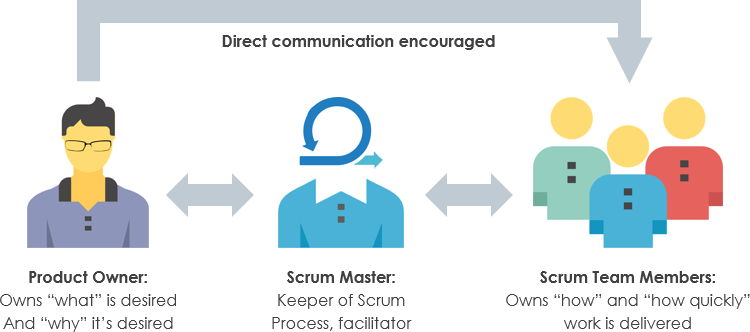
\includegraphics[scale=0.45]{scrum_team.png}}
  \caption{Roles and Responsibilities of the Scrum Team}
  \label{fig:scrum_team}
\end{figure}

The Scrum team of the Tesla Academy project is composed of the following roles:

\begin{itemize}
  \item \textbf{Product Owner}: the academic supervisor and the professional supervisor,
        responsible for the product vision and backlog prioritization;
  \item \textbf{Scrum Master}: the student, responsible for ensuring the proper application
        of the Scrum framework and removing obstacles;
  \item \textbf{Development Team}: the student, responsible for analysis, design,
        development, testing, and documentation.
\end{itemize}

\subsection{The Three Pillars of Scrum}

The Scrum methodology is based on three fundamental pillars that ensure transparency and
effectiveness throughout the development process:

\begin{itemize}
  \item \textbf{Transparency}: all information related to project progress is visible to
        stakeholders;
  \item \textbf{Inspection}: regular events are used to evaluate progress, quality, and
        alignment with objectives;
  \item \textbf{Adaptation}: adjustments are made whenever deviations from the objectives
        are identified.
\end{itemize}

\subsection{Scrum Events}

Scrum relies on a set of structured events that organize the development process:

\begin{itemize}
  \item \textbf{Sprint Planning}: a planning meeting held at the beginning of each sprint
        to select the backlog items to be developed;
  \item \textbf{Daily Scrum}: a short daily meeting used to synchronize work and identify
        obstacles;
  \item \textbf{Sprint Review}: a demonstration of the delivered increment to stakeholders
        at the end of each sprint;
  \item \textbf{Sprint Retrospective}: a continuous improvement meeting used to identify
        what went well and what can be improved.
\end{itemize}

\subsection{Scrum Artifacts}

Scrum artifacts provide transparency and support inspection and adaptation:

\begin{itemize}
  \item \textbf{Product Backlog}: an ordered list of all features, corrections, and
        improvements required for the product;
  \item \textbf{Sprint Backlog}: the subset of Product Backlog items selected for
        implementation during a specific sprint;
  \item \textbf{Increment}: a functional and potentially deliverable version of the product
        produced at the end of each sprint.
\end{itemize}

\subsection{Scrum Life Cycle}

\begin{figure}[htbp]
  \centerline{\includegraphics[scale=0.40]{scrum.png}}
  \caption{Scrum Methodology Life Cycle}
  \label{fig:scrum}
\end{figure}

As shown in Figure~\ref{fig:scrum}, the Scrum cycle begins with the \textit{Product Backlog},
which contains all the features to be developed. For each two-week sprint, a selection of
these features is planned and added to the \textit{Sprint Backlog}. At the end of the
sprint, a functional increment is delivered, tested, and potentially deployable. The Sprint
Review and Sprint Retrospective allow the team to continuously improve both the product and
the development process.

%% ------------------------------------------------------------
\section*{Conclusion}
\addcontentsline{toc}{section}{Conclusion}
%% ------------------------------------------------------------

This chapter established the general framework of the Tesla Academy project. It presented
the host organization, YohaTech Monastir, and described the context that motivated the
development of the platform. The analysis of the existing situation and the benchmark of
competing solutions highlighted the need for a learning platform that combines
multi-organization management, local payment integration, live learning sessions,
assessment tools, AI-powered educational features, and a multilingual orientation adapted
to the Tunisian and regional market.

The chapter also introduced the proposed solution and the Scrum methodology adopted to
organize the development process through iterative and incremental delivery. The next
chapter will focus on the detailed analysis of functional and non-functional requirements
and the planning of the project.
